\documentclass{scrreprt}

% allow images
\usepackage{graphicx}
% allow chinese
\usepackage{CJK}
% lists
\usepackage{enumitem}
% hyperlinked TOC (note the CJKbookmarks boolean)
\usepackage[CJKbookmarks = true]{hyperref}
% allow figures and tables to hold position
\usepackage{float}
% pretty tables
\usepackage{booktabs}
\usepackage[table]{xcolor}
% symbols
\usepackage{gensymb}
% format headers and footers
\usepackage[automark,headsepline,footsepline,plainfootsepline]{scrlayer-scrpage}
% allow for usage of \Blinddocument to test formatting
\usepackage{mwe}
\usepackage{csvsimple}

% options
\graphicspath{{./figures/} {../}}
\definecolor{light-gray}{gray}{0.95}
%% alternate table row colors
\rowcolors{1}{white}{light-gray}

% define macros
\newcommand{\pchapter}[1]{
	\begingroup\let\clearpage\relax
	\newpage
	\begin{figure}[H]
		
\includegraphics[width=0.25\textwidth]{logo.jpeg}
	\end{figure}
	\chapter{#1}
	\endgroup
}
\newcommand{\modelno}{\texttt{WL11M1000}}
\newcommand{\x}{$\times$}
\newcommand{\ptable}[2]{
	\begin{table}[H]
	\caption{#2}
	\centering\csvautobooktabular{#1}
	\end{table}
}

% define header, title, date
\lohead{
\includegraphics[width=\marginparwidth]{logo.jpeg}}
\title{
	\begin{figure}[H]
		\centering
\includegraphics[width=0.5\textwidth]{logo.jpeg}
	\end{figure}
	\vspace{1cm}
	\flushright
	IEEE 802.11 b/g/n 1T/1R IOT Module\\
	\Huge{SPECIFICATION SHEET}\\
	\vspace{2cm}
	\huge{Model No. \modelno}\\
	\vspace{2cm}
		\LARGE{Prepared by David Qiu \\ on behalf of FRUITION CO., LTD.}
}
\date{
	Last revision: February 18th, 2019\\
}
%%%%%%%%%%%%%%%%%%%%%%%%%%%%%%%%%%%%%%%%%%%%%%%%%%%%%%%%%%%%%%%%%%%%%%%%%%%%%%%%
\begin{document}
\begin{CJK*}{UTF8}{gbsn}
\maketitle
\tableofcontents

\pchapter{Product Overview}

\section{General Description}

This document provides the hardware specification of the \modelno\ 802.11b/g/n
1T1R module.  It is based on the MTK MT7682 low-power chipset complied with the
IEEE 802.11n standard, and is backward-complied with IEEE 802.11b/g standards
from 2.4--2.5GHz. It can be used to provide up to 54 Mbps under the IEEE 802.11g
standard, 11 Mbps under the IEEE 802.11b standard, and 150Mbps under the IEEE
802.11n standard.


With seamless roaming and security compliance with the WEP standard, our
\modelno\ 802.11b/g/n module offers absolute interoperability between nearly all
available wireless access points.

\section{Features}

\begin{itemize}
\item Supports all data rates of the IEEE 802.11g standard, including 6, 9, 12,
18, 24, 36, 48 and 54 Mbps.
\item Supports short GI and all data rates of 802.11n including MCS0 to MCS7.
\item Compliant with wireless security protocols WEP, WPA2 and WPS.
\item Supports SoftAP and sniffer modes.
\item Supports MediaTek Smart Connection.
\item Supports multi-cloud connectivity.
\item Interface multiplexing with GPIO.
\item Lightweight TCP/IP protocol.
\item RoHS compliant.
\end{itemize}

\begin{figure}[H]
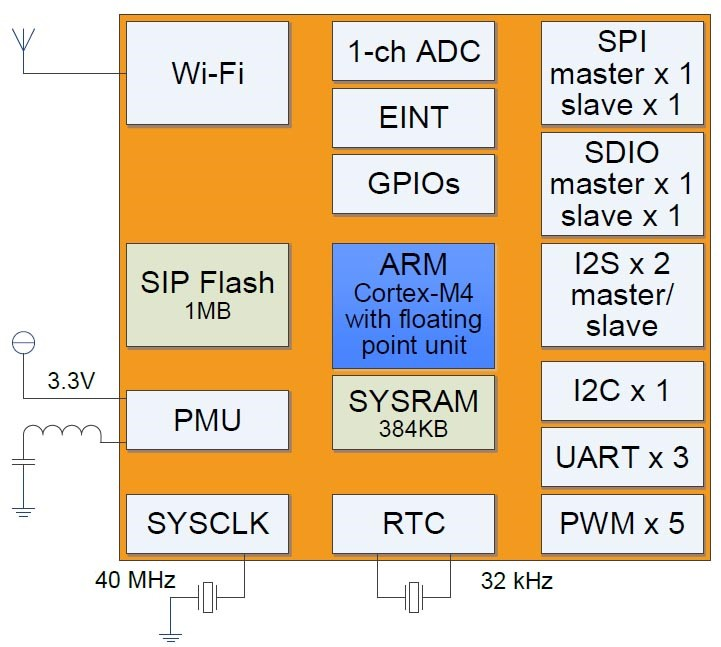
\includegraphics[width=\textwidth]{block.jpg}
\caption{Functional block diagram of the \modelno\ wireless module.}
\end{figure}

\pchapter{Detailed Specifications}

\section{Physical Dimensions}

Size: 12 mm x 12 mm x 0.8 mm.

Weight: 0.4 g

\begin{figure}[H]
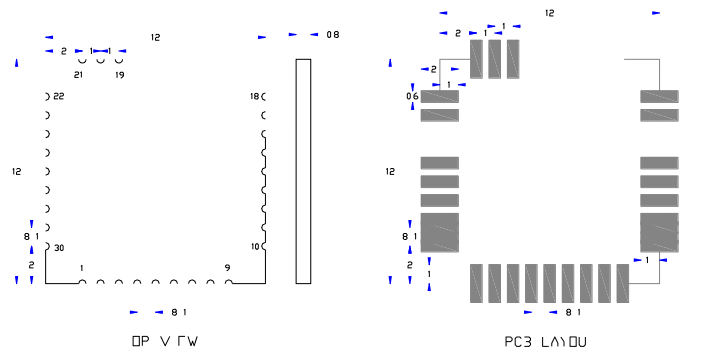
\includegraphics[width=\textwidth]{dimensions.png}
\caption{Dimensions of the \modelno\ wireless module.}
\end{figure}

\section{I/O Specifications}

All data listed below were recorded at 25 \degree C.

Operating voltage: (3.3 $\pm$ 0.3) V

Maximum current usage: 120 mA (RX) or 300 mA (TX)

\begin{table}[H]
\caption{I/O specifications for the \modelno\ wireless module under the IEEE 802.11b standard.}
\centering\csvautobooktabular{figures/80211b_specs.csv}
\end{table}

\begin{table}[H]
\caption{I/O specifications for the \modelno\ wireless module under the IEEE 802.11g standard.}
\centering\csvautobooktabular{figures/80211g_specs.csv}
\end{table}

\begin{table}[H]
\caption{I/O specifications for the \modelno\ wireless module under the IEEE 802.11n standard.}
\centering\csvautobooktabular{figures/80211n_specs.csv}
\end{table}

\section{Memory Specifications}

\begin{itemize}
\item Up to 384 KB SRAM, with zero-wait state, and a maximum frequency of 96 MHz.
\item Up to 32 KB L1 cache with high bit rate, zero-wait state, and a maximum frequency of 192 MHz.
\item Embedded 8 Mbits flash, with less than 0.1 $\mu$A (typical), and a maximum frequency of 80 MHz.
\end{itemize}

\section{Electrical and Thermal Conditions}

\begin{table}[H]
\caption[width=\textwidth]{Temperature limit ratings for the \modelno\ wireless module.}
\centering\csvautobooktabular{figures/ranges.csv}
\end{table}

\pchapter{Programming Interface}

\begin{figure}[H]
\caption{Pin definitions of the \modelno\ wireless module.}
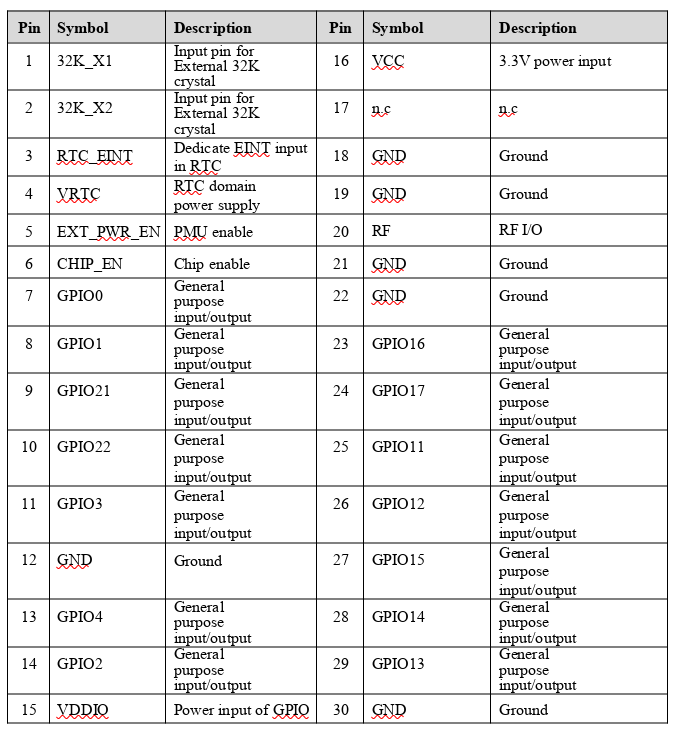
\includegraphics[width=0.8\textwidth]{pin_definitions.png}
\end{figure}

\begin{figure}[H]
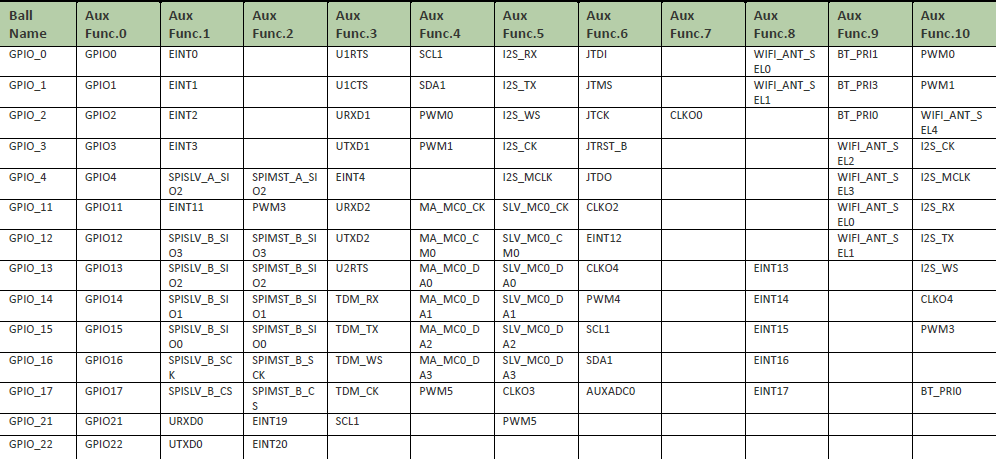
\includegraphics[width=\textwidth]{unknown.png}
\end{figure}

\pchapter{General Recommendations}

\begin{figure}[H]
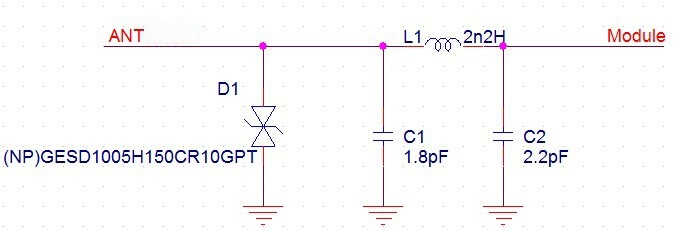
\includegraphics{circuit.png}
\end{figure}

Wireless antennae matching circuits C1, C2, and L1 have been soldered on the
board in advance. Ensure the RF input on the motherboard has an impedance of 50
ohms. It is also not recommended to have a 90 degree cable route, as the cable's
length does not exceed 20 mm.

Reflow profile was determined according to the IPC/JEDEC standard. It is
recommended to use a peak temperature less than 250 \degree C, repeated two or
fewer times.

\begin{figure}[H]
\caption{Recommended reflow profile.}
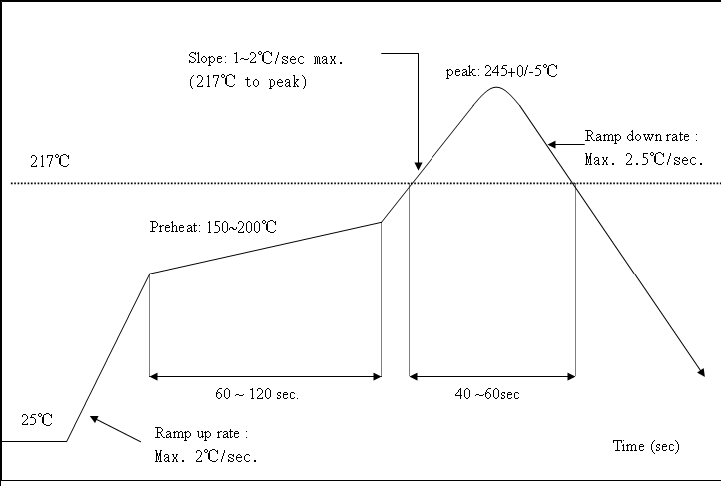
\includegraphics[width=\textwidth]{reflow.png}
\end{figure}

Upon opening the package, it is strongly advised to use nitrile gloves and an
anti-static ring while handling the modules. Generally, it is advised to use a
furnace temperature of 250 \degree C. Limit the module's exposure to humidity
and ambient conditions. The module has a storage life of 12 months, and should
be stored under 40 \degree C and under 90\% humidity. Modules should also be
baked at 125 \degree C for 8 hours to remove excess moisture, improving storage
lifetime. Remember to place dessicant packages following baking.

\pchapter{Module Packaging}

The outer box has dimensions of 426 mm \x\ 378 mm \x\ 220 mm.

The inner box has dimensions of 414 mm \x\ 365 mm \x\ 38 mm.

The anti-static vacuum packaging has dimensions of 360 mm \x\ 430 mm.

Each package contains 7500 pieces a carton, with 5 inner boxes containing 1500
pieces each.

\begin{figure}[H]
\caption{Packaging protocol of the \modelno\ wireless module prior to shipping.}
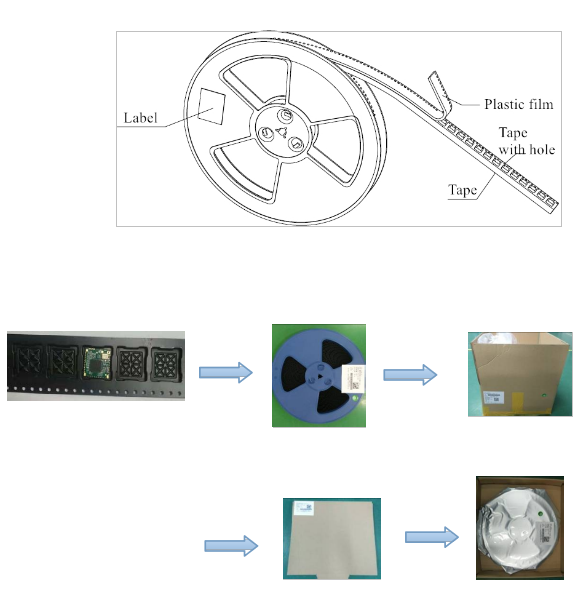
\includegraphics[width=\textwidth]{packaging.png}
\end{figure}

\end{CJK*}
\end{document}
%%%%%%%%%%%%%%%%%%%%%%%%%%%%%%%%%%%%%%%%%%%%%%%%%%%%%%%%%%%%%%%%%%%%%%%%%%%%%%%%
